\chapter{Desarrollo del proyecto : Simulador de juego}

\section {Abstracciones, decisiones y simplificaciones}
\label{sec:abstracciones}

A la hora de plantearse el desarrollo del proyecto, se ha comenzado tomando una serie de decisiones a la hora de diseñar el proyecto. 

La primera decisión procede de la estructura del diseño. La primera decisión tomada con respecto a esto es que el algoritmo funcione como una caja negra para el motor de juego, es decir, que independientemente de cómo sea el funcionamiento del algoritmo no influya para nada en el código del motor de juego. 

Siguiendo este hilo de razonamiento, se ha decidido que el motor de juego y el algoritmo se programen en medios separados, conectados entre ambos y que, cuando el motor de juego lo necesite, se llame al algoritmo para la toma de decisiones mediante esa conexión.
El esquema visual de este planteamiento sería el siguiente:
 
\begin{figure}[h]
\centering
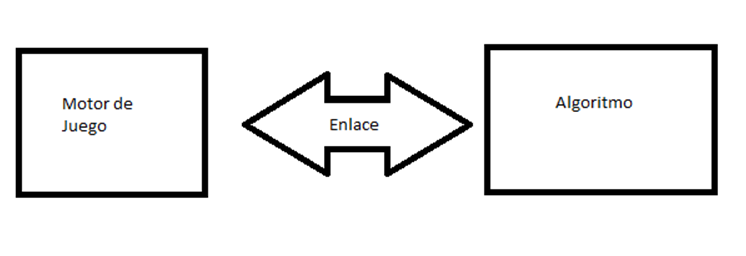
\includegraphics[width=0.45\textwidth]{figuras/esquema.png}   
\caption{Diagrama de diseño del modelo de funcionamiento \cite{propiaPaint}}
\label{fig:esquema}
\end{figure}

Con esta idea en mente, se puede proceder a las elecciones de los medios para programar. En lo que se refiere a los medios utilizados, las elecciones han sido las siguientes:
 \begin{itemize}
\item El motor de juego se ha desarrollado en C++ utilizando Visual Studio 2019. 
\item El algoritmo, las probabilidades y todas las iteraciones se han desarrollado en lenguaje R utilizando la versión R 4.0.0
\item El enlace se ha implementado usando un API REST, con parte programada en C++ y otra en R.
\end{itemize}

Se ha  decidido usar esos lenguajes de programación por comodidad, pues es con los que más tiempo se ha trabajado previamente.

Una vez establecidos los medios a utilizar, es necesario plantearse algunas abstracciones con el fin de simplificar el código a desarrollar, la matemática y, en general, todo el proyecto.

 \begin{itemize}
\item El juego se realizará en la modalidad de \textit{Heads-up}, es decir, el número de jugadores será 2: jugador0 y jugador1. Esta simplificación se hace por varios motivos:
 \begin{itemize}
\item Se limita la información a modelar, ya que las únicas variables ocultas de otros jugadores es un conjunto de 2 cartas.
\item Se limita el número de modelados, ya que solo es necesario modelar a un oponente.
\item Se eliminan factores como la posición con respecto al \textit{Dealer}, lo que facilita desarrollar una estrategia de juego.
\end{itemize}
\item Tal y como se había adelantado en el apartado \ref{sec:choices}, el juego elegido es Texas Hold'em. Como tipo de apuestas, será una apuesta sin límite. En otras palabras, las partidas serán en HUNL(Heads-Up No-Limit) Texas Hold'em.
\item El jueego tendrá dos modos de juego: 
\begin{itemize}
\item Jugador vs Máquina, en el cual un jugador controla al jugador0 para enfrentarse al algoritmo diseñado, que controlará al jugador1. Esta modalidad tiene una funcionalidad principalmente de pruebas de funcionamiento
\item Máquina vs Máquina, en el cual el motor de juego juega solo, que generará un registro con todas las acciones y el resultado de cada mano en beneficio neto. Este modo tiene dos opciones: Algoritmo vs Patrón, donde el Algoritmo se enfrentará a un patrón a la elección del jugador, y Patrón vs Patrón, donde puede hacerse que se enfrenten los Patrones predefinidos entre ellos.
\item El enlace se ha implementado usando un API REST, con parte programada en C++ y otra en R.
\end{itemize}
\item El dinero inicial, así como el valor de la Ciega Grande se podrá introducir manualmente. Para las pruebas de este algoritmo se han utilizado una cantidad constante (10000 de dinero inicial y 20 de ciega grande). Se han tomado estas cantidades a las pruebas para mantener una proporción de 500:1 entre dinero inicial y ciega grande. Cabe destacar que el valor de la ciega grande es una unidad estándar para medir los valores de ganancia en una partida.
\item Los elementos de apuestas relacionados con los casinos se suprimen. Es decir, el \textit{Ante} y el \textit{Rake}. Estos dos elementos no influyen en la probabilidad de las acciones de juego. Si bien el \textit{Ante}  pueda llegar a ser considerado un posible factor a la hora de tomar algunas estrategias, su relevancia solo aparece en situaciones límite, por lo que en la mayoría de los casos solo supone una dificultad añadida a la hora de gestionar las apuestas. Lo mismo pasa con el \textit{Rake}, salvo que este elemento no tiene importancia alguna ni en la probabilidad ni en la estrategia de juego, por lo que lo único que aporta son complicaciones a la hora de programar.
 \begin{itemize}
\item A modo adicional, la eliminación del \textit{Rake} conviere al juego en un juego Suma-Cero, es decir, que las ganancias o pérdidas de un jugador se equilibra perfectamente con las ganancias o pérdidas de los demás jugadores. Al ser un HUNL póker, esto se traduce como las pérdidas de uno de los dos jugadores son las ganancias del otro jugador.
\end{itemize}
\item Se modela el quemado de cartas. Si bien este elemento no influye en la probabilidad ni en la estrategia, es un elemento más del Hold'em y es totalmente inócuo al flujo de juego, por lo que no complica la programación, así que se modela únicamente por similitud con el juego original.
\item Se limita el número de subidas en una misma ronda de apuestas a 3. Esta decision se toma principalmente por optimización de tiempo de ejecución, y para evitar que haya bucles infinitos de cara al modo Máquina vs Máquina.
\item El número de manos máxima será definido al comienzo de las iteraciones, por lo que será un número limitado.
\item La partida acaba cuando ocurra, al menos, una de las siguientes situaciones:
\begin{itemize}
\item El dinero de uno de los dos jugadores llega a 0
\item En el modo de Jugador vs Algoritmo, cuando el jugador desee finalizar la partida.
\item En el modo de Máquina vs Máquina, cuando se alcance el número de iteraciones deseadas.
\end{itemize}
\end{itemize}

\section {Cuantificación de las jugadas}
\label{sec:valmano}

Con el fin de simplificar el cálculo de jugada obtenida, se ha decidido cuantificar las posibles jugadas, otorgándole un valor numérico (usando variables de tipo float en el motor de juego, y un valor entero en el algoritmo)\footnote{Esta diferenciación se hace porque el algoritmo necesita comparar jugadas iguales a la suya, añadiendo el \textit{kicker} haría practicamente imposible el igualar una mano, salvo en contadas ocasiones. En el motor de juego si que es necesario mantenerlo pues es necesario determinar un ganador.} durante el código. También se cuantifica el valor de desempate o \textit{kicker}. Esto permite al código comparar numéricamente  las jugadas de los dos jugadores, y permite establecer si una jugada es superior a otra con bastante facilidad.

Para cuantificar estas jugadas, se ha decidido otorgar un valor entero de 0 a 9 a las distintas jugadas (siendo el 9 la Escalera Real y el 0 Carta más alta). En el simulador se le ha sumado decimales que caracterice el valor dentro de su jugada y la diferencie de otras jugadas del mismo tipo, siempre que sea posible (por ejemplo, en una Escalera, el valor de la carta más alta) e incluya el desempate para cada jugada.  Se ha tomado la decisión de utilizar estos valores para hacer una comparación sencilla de computar (0 a 9, sin necesidad de usar una segunda cifra para las jugadas, y decimales para el desempate, permitiendo comparar de manera más sencilla dos jugadas del mismo tipo).

Se toman estos valores numéricos para poder categorizar las 10 posibles jugadas de manera numérica de una manera uniforme, aunque la frecuencia con la que aparecen dichas manos sea muy diversa, para poder hacer una comparación entre las jugadas. Estos valores podrían tomar cualquier valor, siempre que se mantenga un esquema para diferenciar estas 10 posibles jugadas y poderlas comparar.

Se desarrolla la tabla de la siguiente forma, incluyendo en cada jugada sus correspondientes valores característicos y desempates si aplican.

\begin{longtable}[c]{|c|c|m{3em}|m{8em}|m{8em}|}
\hline
\rowcolor{lightgray} Jugada & Estructura&  Valor Entero & Valor Caract. &  \textit{Kicker}\\ \hline
Escalera Real &9&9&-&-\\
\hline
Escalera de Color&8,AA&8& A = valor de carta más alta x$10^{-2}$&-\\
\hline
Póker&7,AAXX& 7 & A = valor de carta repetida x$10^{-2}$&X = valor de carta más alta fuera de póker x$10^{-4}$ \\
\hline
Full&6,AABB&6&A = valor de carta del trio x$10^{-2}$   B = valor de carta de la pareja  x$10^{-4}$&- \\
\hline
Color &5,AABBCCDDEE&5&A-E = valores del color ordenados de mayor a menor x$10^{-2*i}$&-\\
\hline
Escalera&4,AA&4&A= Valor de la carta alta de la escalerax$10^{-2}$&- \\
\hline
Trío&3,AAXXYY&3 &A = Valor de la carta del trio x$10^{-2}$&X = valor de la carta más alta que no sea del trio x$10^{-4}$ Y= Valor de la segunda carta más alta que no sea del trio x$10^{-6}$ \\
\hline
 Doble Pareja&2,AABBXX& 2 &A = Valor de la carta de la pareja de más valor x$10^{-2}$ B = Valor de la carta de la pareja de menos valor  x$10^{-4}$ &X=valor de carta más alta que no sea de las parejas x$10^{-6}$\\
\hline
 Pareja & 1,AAXXYYZZ & 1& A = Valor de la carta de la pareja x$10^{-2}$&X = valor de la carta más alta que no sea de la pareja x$10^{-4}$ Y= Valor de la segunda carta más alta que no sea de la pareja x$10^{-6}$ Z= Valor de la tercera carta más alta que no sea de la pareja x$10^{-8}$  \\
\hline
 Carta Alta&0,AAWWXXYYZZ & 0& A= valor de la carta más alta x$10^{-2}$&W = valor de la segunda carta más alta x$10^{-4}$ X= valor de la tercera carta más alta x$10^{-6}$ Y= valor de la cuarta carta más alta x$10^{-8}$ Z= valor de la quinta carta más alta x$10^{-10}$ \\
\hline
\caption{Formato del valor de las jugadas en Texas Hold'em}
\label{tab:kicker}
\end{longtable}


\section {Desarrollo del Motor de Juego}
\label{sec:motor}

Para el simulador de juego, en lenguaje C++, se han creado varias clases para estructurar el código, clases en las que se profundizará en su respectivo apartado. Las clases son las siguientes:

 \begin{itemize}
\item Carta: clase base que clasifica palo, número y tiene una función para imprimir la carta por pantalla. 
\item Jugador: tiene un array de Carta (para representar las manos), funciones para gestionar su dinero y sus apuestas, así como funciones para calcular el valor de su jugada.
\item Mesa: tiene dos arrays de Carta (para representar el tablero y las cartas quemadas) y tiene tanto las funciones de gestionar los índices de la partida como de imprimir el tablero en cada ronda.
\item Mazo: tiene un array de Carta y un índice para representar la posición de las cartas. También tiene las funciones para barajar el mazo (aleatorizando la posición de las cartas) y repartir las cartas tanto a jugadores como a la mesa.
\item Algoritmo: que contiene las distintas funciones para comunicarse con el algoritmo, así como los elementos para gestionar los distintos patrones.
\item Random: Que incluye toda la programación del generador de números pseudoaleatorios Keep It Simple Stupid (KISS), así como las funciones para generar números aleatorios (tanto valores porcentuales como en enteros).
\end{itemize}

Además de eso, está el archivo principal (Póker\_Simu.cpp) que inicializa los elementos de las clases y contiene un array de objetos Jugador, englobando los dos jugadores, un elemento de tipo Mesa que representa la mesa de juego. Además, Poker\_Simu.cpp tiene todas las funciones del que participan en el flujo de la ronda de juego,las funciones de las rondas de apuestas de cada uno de los modos y las funciones para determinar ganadores

\subsection{Clase Carta}
\subsubsection{Atributos}

Cada elemento de la clase carta tiene los siguientes atributos de tipo protected:
 \begin{itemize}
\item \textit{Palo (int)}: un valor de tipo int que representa el palo de la carta. Puede adquirir los valores de 1 (Tréboles), 2 (Picas), 3 (Diamantes) y 4 (Corazones).
\item \textit{Numero (int)}: un valor de tipo int que representa el valor de la carta. Puede adquirir los valores de 1 a 13, aunque algunas funciones pueden sustituir el valor de 1 por 14 para el tema de cálculos, siendo 1 (o 14) el valor para As, 11 para J, 12 para Q y 13 para K.
\end{itemize}

Con estos dos atributos, se pueden caracterizar cualquiera de las 52 cartas de la baraja francesa, como, por ejemplo:

\begin{longtable}[c]{|c|c|c|}
\hline
\rowcolor{lightgray}Carta de la baraja &Numero&Palo\\
 \hline
9$\spadesuit$&9&2\\
\hline
\textcolor{red}{3$\varheartsuit$}&3&4\\
\hline
J$\clubsuit$&11&1\\
\hline
\textcolor{red}{9$\vardiamondsuit$}&1 ó 14 (según la función)&3\\
\hline
\caption{Ejemplos de Atributos Carta}
\label{tab:carta}
\end{longtable}

\subsubsection{Funciones}
En esta clase se recogen las siguientes funciones:
\begin{itemize}
\item \textit{Int GetPalo() / int GetNumero()}: Dado que los atributos son de tipo protected, se leen utilizando una función que tenga como salida dichos atributos.
\item\textit{ Void SetPalo(int p) / void SetNumero(int n)}: Al igual que pasa a la hora de leer los atributos, para poder modificarlos es necesario una función para poder modificarlos, dejando como valor nuevo el valor int de entrada.
\item \textit{Void imprimirCarta()}: Esta función lee los valores numéricos de los atributos de Carta e imprime una frase en función del número y el palo de cada carta.
 \end{itemize}

\subsection{Clase Jugador}
\subsubsection{Atributos}

En esta clase se incluyen los siguientes atributos:
\begin{itemize}
\item \textit{mano}: un Array de dos elementos de tipo Carta, que representan las dos cartas iniciales que tiene el jugador.
\item \textit{apuesta} y \textit{apuestaInicial}: atributos de tipo float que representan las dos apuestas del jugador, siendo apuestaInicial el valor de la Ciega que le toque apostar, y apuesta el valor de la apuesta de esa ronda.
\item \textit{Dinero}: atributo de tipo float que indica el dinero restante del jugador.
\item Conjunto de \textit{Valores\_Mano}: son 4 atributos de tipo float que representan el valor numérico de la jugada  que se tiene durante la ronda correspondiente (valor\_mano-$>$Preflop, valor\_mano\_r1-$>$Flop, valor\_mano\_r2-$>$Turn y valor\_mano\_r3-$>$River), siguiendo el esquema del apartado 3.2.
\item Conjunto de \textit{jugada\_obtenida}: son 9 atributos de tipo bool que representan qué jugada se ha obtenido, de modo de ayuda para el posterior cálculo del valor numérico.
\item\textit{ Valor\_num\_mano}: un atributo de tipo float que representa el valor numérico de la mano, para cálculos de desempate.
\end{itemize}

\subsubsection{Funciones}
Por una parte, en esta clase se tienen los siguientes pares de funciones Set() y Get(), para modificar y obtener, respectivamente el valor de dicho atributo:
\begin{itemize}
\item \textit{Carta* getMano()/setMano(Carta* c)}
\item \textit{Float getDinero()/setDinero(float f)}
\item\textit{ Float getApuestaInicial() / setApuestaInicial(float f)}
\item \textit{Float getValor()}
\item \textit{Float getApuesta () / setApuesta (float f)}: aquí cabe destacar que setApuesta obtiene la diferencia entre la apuesta actual y f, asigna el valor de f a apuesta y después hace un \textit{setDinero(dinero\_actual – diferencia).}
 \end{itemize}
Por otro lado, se tienen un conjunto de funciones Reset, cuya función sirve para devolver al estado original algunos de los atributos de la clase:
\begin{itemize}
\item \textit{resetObtenidas()}: para poner cada una de las variables del conjunto de jugada\_obtenida con el valor inicial de false.
\item \textit{ resetApuesta()}: para convertir el valor de apuesta en 0.
\item \textit{resetBool()}: para poner cada una de las variables del conjunto de jugada\_obtenida con el valor inicial de true.
 \end{itemize}
Además, se tienen las funciones del cálculo del valor de la mano:
\begin{itemize}
\item \textit{valorManoInicial()}: Utilizando la fórmula de Chen, obtiene una valoración numérica de la mano inicial durante  el Preflop.
\item \textit{valorManoR1(mesa T)/ valorManoR2(mesa T)/ valorManoR3(mesa T)}: que calcula para cada ronda el array de cartas correspondiente para dicha fase (unión de Mano y las cartas del tablero disponibles esa ronda), ordena las cartas de mayor a menor y ejecuta calculoValorJugada introduciendo como entrada ese array y un valor numérico (5, 6 o 7), en función de la ronda..
\item \textit{calculoValorJugada(carta* c, int i)}: recibiendo el array de cartas ordenadas c y un índice numérico para identificar qué ronda de juego es, hace el cálculo del valor numérico. Para ello primero contabiliza los siguientes datos:
\begin{itemize}
\item Nº de cartas repetidas: identifica si hay cartas repetidas, cuantas veces se repite una carta, el número de dicha carta y el número de cartas distintas repetidas, si los hubiera.
\item Nº de palos repetidos: identifica cuántas cartas pertenencen a cada palo. 
\item Nº de cartas consecutivas: identifica cuántas cartas consecutivas hay en el array.
 \end{itemize}
 \end{itemize}
Ahora se procede a analizar los tipos de jugada posibles y como estos tres datos son necesarios para cada una, creando esta tabla:

\begin{longtable}[c]{|c|m{8em}|m{8em}|m{5em}|}
\hline
\rowcolor{lightgray}Jugada\textbackslash Dato&Cartas Repetidas& 5 Cartas consecutivas & 5 Cartas del mismo palo\\
\hline
Escalera Real&No&Si (10-A)& Si\\
\hline
Escalera de Color&No&Si (distinto de 10-A)& Si\\
\hline
Poker&Si (4 Cartas iguales)& No & No\\
\hline
Full&Si (3 Cartas repetidas y otras dos repetidas distintas)& No & No\\
\hline
Color&No& No & Si\\
\hline
Escalera&No& Si & No\\
\hline
Trio&Si (Tres cartas repetidas)& No & No\\
\hline
Doble Pareja&Si (4 cartas repetidas dos a dos)& No & No\\
\hline
Pareja&Si (2 cartas repetidas)& No & No\\
\hline
Carta Alta&No& No & No\\
\hline
\caption{Datos necesarios para cada jugada}
\label{tab:tabla}
\end{longtable}

A partir de los datos necesarios de esta tabla y, en función de los datos obtenidos, comienza el cálculo de la mejor jugada. Primero analiza qué jugadas se han obtenido, asignando el valor true a la variable correspondiente. 
\begin{itemize}
\item En caso de que haya cartas repetidas, se almacena cuantas cartas hay repetidas y qué número de carta es el repetido. Teniendo en cuenta que son 7 cartas máximo de donde se tienen que obtener la mejor jugada (En River están las cinco cartas de la mesa más las dos que tiene el jugador), el máximo de repeticiones distintas son 3 repeticiones distintas. En función de cuantas cartas obtenidas, se dará valor true a las variables póker\_obtenida, full\_obtenida, trio\_obtenida, doble\_pareja\_obtenida y/o pareja\_obtenida.
\item Si uno de los palos repetidos tiene 5 o más cartas de ese palo, el jugador ha obtenido Color. En ese caso, almacena las cartas del palo en un array auxiliar para el color y se da el valor color\_obtenida=true.
\item Si hay, al menos, cinco cartas consecutivas, se ha obtenido Escalera. También considera el caso concreto de tener 5, 4, 3, 2 y A, que también es considerado escalera debido al valor doble del As. En caso afirmativo, almacena las cartas consecutivas en un array auxiliar para la escalera y se da el valor escalera\_obtenida=true
\item Si se da la situación en la que haya tanto 5 cartas consecutivas como 5 cartas del mismo palo, es decir ocurra  escalera\_obtenida == true y color\_obtenida == true, se comparan los arrays auxiliares y, si coinciden al menos 5 cartas, se ha obtenido una Escalera de color, dando el valor escalera\_color\_obtenida=true.
\item Si se da escalera\_color\_obtenida=true, se compara la escalera con los valores establecidos de la Escalera Real (A, K, Q, J, 10). Si coinciden esas 5 cartas con las de la escalera de color, se habrá obtenido la Escalera Real dando el valor de escalera\_real\_obtenida = true
 \end{itemize}

De esta manera, se habrá contemplado la posibilidad de cualquiera de las 9 jugadas que requieren alguna combinación de cartas (es decir, cualquier jugada que no sea “Carta alta”).
\begin{figure}[h]
\centering
\includegraphics[width=0.75\textwidth]{figuras/grafo1.png}   
\caption{Asignación de jugada\_obtenida en función de los datos obtenidos en de la jugada.\cite{propiaCreately}}
\label{fig:jugada_ob}
\end{figure}

Una vez determinados los atributos del conjunto jugadas\_obtenidas que tienen valor true, se determina mediante condiciones if la mejor jugada, y se calcula el valor de desempate, siguiendo las guias que aparecen en la tabla \ref{tab:kicker}
Se han creado los diagramas \ref{fig:jugada_ob} y \ref{fig:valor} para que sea más visual esta explicación de funcionamiento.


\begin{figure}[h]
\centering
\includegraphics[width=0.75\textwidth]{figuras/grafo2.png}   
\caption{Asignación del valor jugada correspondiente en función de jugada\_obtenida. \cite{propiaCreately}}
\label{fig:valor}
\end{figure}

Por último, se tiene la función de \textit{imprimirMano()}, para ejecutar la función \textit{imprimirCarta()} de cada una de las cartas de la mano del oponente.


\subsection{Clase Mesa}
\subsubsection{Atributos}

La clase mesa se compone de los siguientes atribuitos:
\begin{itemize}
\item Índices: son 4 atributos de tipo int, que representan índices para el flujo del juego:
\begin{itemize}
\item  \textit{indiceRonda} se utiliza para llevar el conteo de la fase de la ronda (0 para preflop, 1 para flop, 2 para turn, 3 para river y 4 para showdown).
\item  \textit{indiceTablero} indica la siguiente posición del array Tablero.
\item  \textit{indicieQuemada} indica la siguiente posición del array Quemada.
 \end{itemize}
\item Arrays de carta: son dos array de atributo Carta:
\begin{itemize}
\item  \textit{Tablero:} array de 5 elementos, que sirve para almacenar las cartas que son visibles para ambos jugadores
\item  \textit{Quemada:} array de 3 Cartas, que sirve para almacenar las cartas que se “queman”
 \end{itemize}
\item  \textit{Apuesta:} float que representa la suma total de las apuestas de los jugadores.
\item  \textit{Tablero\_juego\[11\]\[26\]:} matriz de elementos Char para la representación gráfica de la mesa de juego en el modo de jugador vs algoritmo.
\item  \textit{bool modoJ:} booleano auxiliar que adquiere el valor de TRUE si se está ejecutando el modo jugador vs Máquina.
 \end{itemize}

\subsubsection{Funciones}
Los procesos de la clase Mesa son los siguientes:
\begin{itemize}
\item Funciones de índices: un conjunto de 3 funciones para cada uno de los índices, una función reset para dejar el valor a 0, una función up que aumenta el valor en uno y una función get, para obtener el valor de ese índice:
\begin{itemize}
\item \textit{void resetIndiceTablero(),	void upIndiceTablero() y int getIndiceTablero()}: para el indiceTablero.
\item \textit{void resetIndiceQuemada(),	void upIndiceQuemada() y int getIndiceQuemada()}: para el indiceQuemada.
\item \textit{void resetIndiceRonda(),	void upIndiceRonda() y int getIndiceRonda()}: para el indiceRonda.
 \end{itemize}
\item Funciones de tablero\_juego: son las tres funciones que se encargan de gestionar todo lo relacionado con la presentación visual del juego:
\begin{itemize}
\item \textit{creaTablero():} asigna el valor ‘ ‘ a cada uno de las posiciones de la matriz.
\item\textit{ modificaTablero(jugador* J):} modifica los valores de las posiciones de la matriz para que se adapte a lo que debe mostrar en cada ronda:
\begin{itemize}
\item Preflop: Las dos cartas de la mano del Jugador
\item Flop: Las dos cartas de la mano del Jugador y las tres primeras cartas de Tablero.
\item Turn: Las dos cartas de la mano del Jugador y las cuatro primeras cartas de Tablero.
\item River: Las dos cartas de la mano del Jugador y las cinco cartas de Tablero.
\item Showdown: Las dos cartas de la mano de cada Jugador, las cinco cartas de Tablero y las tres cartas de Quemada.
 \end{itemize}
\item \textit{imprimirTablero(jugador* J) }imprime por pantalla cada uno de las posiciones de tablero\_juego, así como si un jugador ha hecho All In.
 \end{itemize}
\item Funciones de flujo de rondas: son las funciones que están relacionadas con el funcionamiento de las rondas en lo que se refiere a las variables de Mesa
\begin{itemize}
\item \textit{entregarApuesta(jugador J):} se entrega el valor de la apuesta total al jugador J, así como reinicia el valor de apuesta.
\item \textit{actualizarApuesta(jugador* J):} actualiza el valor de apuesta en función de la apuesta de cada uno de los jugadores incluidos en J.
\item \textit{finRonda(Mazo m):} reinicia el valor de apuesta y ejecuta todos los resetIndice.
 \end{itemize}
\item Funciones de conversión a Char: transforma en char los valores de número y palo de la carta C para las funciones de tablero\_juego siguiendo este criterio:
\begin{itemize}
\item \textit{Char conversorNumero(Carta c) }según el valor de getNumero() de c
\item \textit{Char conversorPalo(Carta c) }según el valor de getPalo() de c
 \end{itemize}
\item \textit{Bool continuar():} una vez acaba una ronda pregunta al jugador si desea seguir jugando o terminar el juego. 
 \end{itemize}

\subsection{Clase Mazo}
\subsubsection{Atributos}
Esta clase incluye dos atributos:
\begin{itemize}
\item \textit{Deck:} Un array de elementos Carta de tamaño 52 (representando el mazo de juego)
\item\textit{ indiceMazo:} valor int que representa el índice en el que se está trabajando dentro de Deck
\end{itemize}
\subsubsection{Funciones}
El constructor de la clase,\textit{ Mazo()}, inicializa el mazo y asigna valores de palo y numero a cada uno de los elementos de deck.
Las dos funciones que interactúan con el funcionamiento de la ronda son las siguientes:
\begin{itemize}
\item \textit{Barajar():} aleatoriza el orden de los elementos de deck utilizando los valores generados por la clase Random.
\item \textit{repartirCartas(Mesa T, Jugador* J)}: asigna el valor de las cartas tanto a cada elemento de J como a los arrays Tablero y Quemada de T.
\end{itemize}

Por último, está la función  \textit{resetIndiceMazo()}, que asigna el valor 0 al indiceMazo.


\subsection{Clase Random}
\subsubsection{Definiciones de valores}

Como se comentó en la explicación del algoritmo KISS, es necesario definir los valores que va a utilizar el algoritmo, así como los valores de las semillas. Se van a utilizar las siguientes definiciones de valores para el algoritmo.   \cite{kiss2, kiss1}
\begin{verbatim}
typedef uint64_t u64;

#define QSIZE 0x200000
#define CNG (cng = 6906969069ULL * cng + 1234567)
#define XS (xs ^= (xs<<13), xs ^= (xs>>17), xs ^=(xs<<43))
#define KISS (B64MWC() + CNG + XS)

static u64 QARY[QSIZE];
static int j;
static u64 carry;
static u64 xs;
static u64 cng;
\end{verbatim}

\subsubsection{Definiciones de valores}
Habiendo definido los valores de funcionamiento del algoritmo KISS, se pueden definir las funciones de sta clase. Primero,tiene 6 funciones que sirven para generar los números pseudoaleatorios: \cite{kiss2,kiss1}
\begin{itemize}
\item \textit{int func():} genera un número entero para la función de calentamiento.
\item\textit{ rankd\_reset():} reinicia la semilla de KISS.
\item\textit{u64 B64MWC():} función que genera un número pseudoaletorio usando el método de la multiplicación con acarreo.
\item\textit{randk\_seed():} inicia el generador KISS con la semilla inicial.
\item\textit{ randk\_seed\_manual(u64 seed)} inicia el generador KISS con la semilla introducida.
\item\textit{ u64 randk()} genera un número pseudoaleatorio usando el generador KISS.
\item\textit{randk\_warmup(int rondas):} ejecuta randk() tantas veces como el número de rondas introducido, sin devolver ningún valor, lo cual hace que la secuencia avance.
 \end{itemize}
Tras eso, se tienen las 2 funciones para generar números usando ese algoritmo en el formato que resulta de utilidad para el código (ya que KISS trabaja con valores ULL).
\begin{itemize}
\item \textit{Float nrandomPorcert():} genera un número comprendido entre 0 y 1 utilizando el algoritmo.
\item\textit{ Float nrandomN(int n):} genera un número comprendido entre 0 y n.
 \end{itemize}

\subsection{Clase Algoritmo}
\label{sec:algmoto}
\subsubsection{Atributos}


Los atributos de esta clase incluye el valor \textit{int tipo}, que representa el patron o el algoritmo elegido (que se selecionará en la función Main de Póker\_simu.cpp, descrito más abajo), el valor \textit{ bool pasa}, que representa cuando el algoritmo ha decidido pasar, y el \textit{int acción}, que representa qué acción ha sido la última en tomar el algoritmo (0=pasar, 1=ver, 2=subir).
Por último, se tiene el atributo \textit{triple}, que es un array de 3 números float. Este array representa cómo de probable es que el algoritmo decida tomar una de las tres decisiones. 

\subsubsection{funciones}

Las funciones de la clase algoritmo se encargan de gestionar la toma de decisiones: tanto la recepción de los valores de triple como su transformación en una acción a tomar.

Lo primero es recibir los datos por parte del código R. Para ello, se cuenta con las funciones \textit{obtenerTriple(Jugador J, Mesa M), obtenerTripleAccion(Jugador J, Mesa M, int accionprevia)} y \textit{obtenerTripleAct(jugador J, mesa M, int accionprevia)} que se encargan de comunicar con el código R cada ronda en función de si es la primera toma de decisiones de la ronda siendo jugador inicial, sin ser jugador inicial o si no es la primera toma de decisiones de esa ronda de apuestas respectivamente.

Posteriormente, se tienen las funciones \textit{int obtenerAccion(Jugador J, Mesa M), int obtenerAccionSegundo(Jugador J, Mesa M, int accionprevia)} e  \textit{int obtenerAccionAct(jugador J, mesa M, int accionprevia) }que se encargan de devolver la acción a tomar en función de si es la primera toma de decisiones de la ronda siendo jugador inicial, sin ser jugador inicial o si no es la primera toma de decisiones de esa ronda de apuestas respectivamente.

Para ello, lo primero que comprueba es el atributo tipo. Si es el correspondiente al algoritmo, llamará a la correspondiente función \textit{obtenerTriple} y calculará aleatoriamente cuál de las acciones es la elegida. En caso de que corresponda a uno de los patrones, seguirá el patrón correspondiente para aleatorizar una acción a tomar.

Además de esto, se tienen dos funciones auxiliares que sirven para comunicar al algoritmo que su adversario ha visto la apuesta o ha pasado la apuesta. Estas funciones son \textit{void actualizaBayes(int ronda)} y \textit{void pasar(int ronda)}, respectivamente, donde ronda es la ronda en la que han pasado.

Por último están las funciones \textit{reseteo() }(que devuelve los valores de la clase algoritmo a su estado inicial, así como ejecuta la función reset en el código R) y la función\textit{ float obtenerSubida(float apuesta)}, que devuelve la subida correspondiente a esa apuesta.

\subsection{Poker\_Simu.cpp}
\label{sec:pokersimu}
Dado que este archivo es el que engloba todas las demás funciones restantes, se va a explicar función a función.

\subsubsection{int main()}

La función que inicializa los elementos de cada clase:
\begin{itemize}
\item Mesa Tablero.
\item Mazo mazo.
\item Jugador* Jugadores, un array de dos jugadores (ya que el programa está diseñado para dos jugadores).
\item Algoritmo alg.
\item Bool jugador e int parámetro: valores para determinar el modo de juego y, en caso del modo Algoritmo, el algoritmo elegido.
\item Float bidaux, que sirve para almacenar el valor de la apuesta inicial.
 \end{itemize}
El valor de bool es la salida de \textit{SeleccionarModo()} y el valor int de parámetro es la salida de \textit{SeleccionarAlgoritmo().}
Con todos estos valores, se ejecuta \textit{float iniciarPartida(Tablero, mazo, Jugadores)} y \textit{jugarPartida(Tablero, mazo, Jugadores, jugador, parámetro, alg, bidaux).}

\subsubsection{Bool SeleccionarModo() e int SeleccionarAlgoritmo}
Estas dos funciones sirven para seleccionar el modo de juego (Jugador vs Máquina o Máquina vs Máquina) y el algoritmo predefinido al que se va a enfrentar el patrón programado (Maniaco, Roca o Calling Station) o la combinación de los 3 patrones que se van a enfrentar.
En el caso \textit{bool SeleccionarModo()} devuelve true si el modo Jugador vs Algoritmo es elegido, si no, devuelve false.
En el caso de \textit{int SeleccionarAlgoritmo()} puede devolver los siguientes valores:
\begin{itemize}
\item 1-$>$Algoritmo vs Maniaco.
\item 2-$>$Algoritmo vs Roca.
\item 3-$> $Algoritmo vs Calling Station
\item 5-$>$ Maniaco vs Roca
\item 10-$>$ Calling Station vs Maniaco
\item 13-$>$ Roca vs Calling Station
 \end{itemize}

\subsubsection{IniciarPartida(MesaT, mazo M, Jugador* J) y apuestaInicial(Mesa T, Jugador* Jugadores)}

\textit{IniciarPartida(MesaT, Mazo M, Jugador* J)} tiene la utilidad de inicializar los parámetros de la partida.
Mediante una entrada de valor numérico, se obtiene la cantidad de dinero inicial que tiene cada jugador, usando ese valor se modifica. la cantidad de dinero de cada uno de los jugadores de J con \textit{setdinero()}.
Se ejecuta la función\textit{ creaTablero()} de T para inicializar la mesa de juego y se ejecuta la función \textit{apuestaInicial(Mesa T, Jugador* Jugadores)}.
\textit{apuestaInicial(Mesa T, Jugador* Jugadores)} es una función que sirve para inicializar el valor de la Ciega Grande, así como el valor de la ciega Pequeña y asignárselo a los jugadores mediante \textit{setApuestaInicial(float)} para la ciega grande y \textit{setApuestaInicial(float/2)} para la ciega pequeña. Para hacer esta asignación, primero determina qué jugador será el jugador inicial de manera aleatoria.

\subsubsection{jugarPartida(MesaT,Mazo M, Jugador* J) y apuestaInicial(Mesa T, Jugador* Jugadores)}

Esta función es la que controla el flujo de las fases de cada ronda.
Una vez inicializadas las variables necesarias para la función, incluyendo obtener la apuesta inicial de cada uno de los jugadores y asignar al atributo tipo de alg el valor 4 (el que corresponde al algoritmo diseñado y no a uno de los patrones), determina el flujo de juego según el modo en función del valor del booleano jugador. 

\begin{itemize}
\item Modo Jugador vs Máquina

Esta modalidad tiene una doble función. La primera función es comprobar el correcto funcionamiento del conjunto de motor de juego, enlace y algoritmo, por lo que se usará esta modalidad como herramienta de testeo del algoritmo. La segunda función es comprobar las reacciones del algoritmo ante el factor humano.
Comienza el bucle de juego (controlado por la variable booleana continuar) inicializando los índices de ronda y Mazo, se aleatoriza el mazo con \textit{M.barajar()}, se obtienen las apuestas iniciales, se reparten cartas con \textit{M.repartirCartas(Mesa T,Jugador* j)}, se modifica el tablero y se actualiza la apuesta, incluyendo la alternación de apuestas iniciales en función del jugador inicial. Tras eso, se ejecuta la función \textit{ronda(Mesa T, mazo M, Jugador* J)}, que es la función que representa la fase de apuestas, de la cual se explicará su funcionamiento en su apartado. 
La función ronda devuelve un valor int , que se almacena en la variable int pasar. Tras esto, en función del valor de pasar, se comienza un ciclo de funcionamiento guiado por el valor de pasar y por el valor de indiceRonda (almacenado en auxRonda).
Este segundo bucle incluido en el primero consiste en primero una comprobación del valor de pasar. Si pasar es distinto de 0, ejecuta pasar\textit{Apuesta(Mesa T, Jugadores* Jugadores)} y almacena el resultado en la variable continuar. Si no, continua el ciclo: aumenta tanto índiceRonda (con \textit{T.upIndiceRonda()}) como auxRonda y comprueba el valor de IndiceRonda:
\begin{itemize}
\item Si el valor de IndiceRonda es 4, se procede a hacer el Showdown, es decir, se modifica el tablero, se actualiza la apuesta y se imprime el tablero, revelando todas las cartas y calculando el jugador que gana. Tras determinar el ganador, se entrega la apuesta al ganador y, si ninguno de los jugadores está a 0 de dinero, pregunta al jugador si quiere continuar jugando con T.continuar(), cuya salida se almacena en continuar.
\item Si el valor de IndiceRonda no es 4: se ejecuta de nuevo la función ronda(Mesa T, Carta* c, Jugador* J), que vuelve a almacenar su salida en pasar.
 \end{itemize}
Después de acabar ese ciclo, se continua el ciclo principal, que comprueba si realmente el valor de continuar es correcto debido a un All In y uno del os jugadores no ha perdido.
Este ciclo se repite mientras que continuar==true. Después de eso, imprime por pantalla el ganador.

\item Modo Máquina vs Máquina

Esta modalidad de juego es la que se va a utilizar para analizar la fuerza del algoritmo, ya que permite automatizar n rondas de juego, siendo n un número definido.
El funcionamiento de este modo es bastante similar al modo jugador vs algoritmo. 
Se produce la inicialización de variables: se crea un nuevo elemento de clase Algoritmo llamado \textit{algOpo}, y asigna los valores de tipo para ambos algoritmos en función de  \textit{elegido}:
\item 1-3 -$>$ tipo de alg=4 y tipo de algOpo el valor de \textit{elegido}.
\item 5-$>$ tipo de alg=1y tipo de algOpo =2.
\item 10-$>$ tipo de alg=3y tipo de algOpo =1.
\item 13-$>$ tipo de alg=2y tipo de algOpo =3.
, y se crean los elementos relacionados con el registro de las iteraciones usando fstream y creando un elemento string llamado acciones y un vector de elementos string llamado log, que será el que se acabe pasando al registro. 

También se crean las variables auxiliares necesarias (dos variables \textit{Carta*, manoAux} y \textit{MesaAux}, dos variables int, \textit{status} y \textit{p}, y un string, \textit{cadena\_aux}).
Antes de empezar el ciclo, se pide introducir el número de iteraciones deseadas, lo cual sirve como un elemento a comprobar para salir del bucle de juego.
Se definen las apuestas iniciales de cada jugador, se reparten las cartas y se actualiza la apuesta de la mesa. Después de eso, se realizan la inicialización del registro. 
Para poder analizar como de fuerte es el algoritmo, es necesario llevar un registro de cada iteración. Para ello, la mejor forma de observarlo es con la variación de dinero que tenga el algoritmo. Pero esto se puede analizar de dos formas: en cada iteración o en cada partida. Teniendo en cuenta que la variación de dinero en cada ronda es influida directamente por cómo de buena sea la jugada del algoritmo durante esa iteración, considero que es mejor analizar el beneficio en cada iteración ya que se puede crear una comparación del beneficio con la fuerza de la mano.
La estructura de cada línea del registro es la siguiente:

\textit{\textbf{It: n Time: t \/\/ Mano alg: C1C2 Mano patron: C3C4 \/\/ RX \/\/ SH}}

Siendo n el número de la iteración, t el registro de fecha y hora en el que se inicia dicha iteración (para llevar un registro del tiempo que se tarda por iteración), Ci las correspondientes cartas que tendría en su mano el algoritmo y el patrón elegido, respectivamente, RX la información de las rondas de juego de esa iteración y SH la información del resultado de la iteración
La estructura de RX varía según si es la ronda 0 o cualquiera de las posteriores. La estructura es la siguiente:

\textit{\textbf{Rn Mesa Mi JiAJdA \/\/}}

Siendo n el número de la ronda, Mi las cartas que se encuentran en la mesa durante esa ronda y JiAJdA son las acciones que toma cada jugador (siendo JiA la acción del jugador inicial y JdA la acción del jugador que no es mano inicial, aka dealer). Las acciones pueden ser V (para ver la apuesta), P (al pasar la apuesta) o SX (para el caso de la subida, siendo X el valor de subida). JiAJdA se repetirá tantas veces como sea necesario hasta que ambos jugadores ven la apuesta o uno de los jugadores pasa.
El cambio de esa estructura para la ronda 0 (preflop) es la sección de Mesa Mi, ya que esa sección no aparecerá en esa ronda, mientras que para el resto de las rondas sí que aparecerá. 
Por último, se tiene el valor SH, que representa el resultado final de la partida. La estructura de SH es la siguiente

\textit{\textbf{J1RJ2O s B}}

Siendo R y O el resultado de cada jugador, s el signo asociado al resultado del algoritmo y B la variación en valor absoluto de dinero del algoritmo. Los valores que pueden tomar son W (en caso de que haya ganado), L (en caso de que pierda) o T en caso de empate. Cabe destacar que las únicas combinaciones son J1WJ2L (en caso de que el algoritmo gane), J1LJ2W (en caso de que el patrón gane) o J1TJ2T, ya que ambos empatan. En caso de que el algoritmo gane, s será “+” y B tomará el valor de la diferencia entre la apuesta total y la apuesta hecha. En caso de que el algoritmo pierda, s será “- “y B será la apuesta que tenga el algoritmo, y en el caso de empate, s será “=” y B será la diferencia entre la mitad de la apuesta total y la apuesta hecha.
Se inician tanto el ciclo principal como el secundario, que tendrán una dinámica prácticamente idéntica a la que tienen en el modo Jugador vs Algoritmo, aunque añadiendo la funcionalidad del registro y que se llamará a las funciones equivalentes de las funciones mencionadas para este modo. Cabe destacar que se determinará qué algoritmo ha pasado durante la iteración (en caso de que eso ocurra) usando la variable \textit{pasa} de los elemento Algoritmo.
La parte final del ciclo principal es la que varía, ya que las únicas dos posibilidades para que se dé el valor continuar=false son que uno de los dos jugadores se haya quedado a 0 de dinero o que se haya alcanzado el número definido de iteraciones.

\end{itemize}
\subsubsection{Funciones de ronda y CalcularValorjugador(Mesa T, Jugador* J, int Ronda))}

\textit{int ronda(mesa t, mazo M, jugador* j, Algoritmo alg)} tiene como objetivo modificar el tablero con el índice de ronda correspondiente, calcular el valor de Jugada del jugador con \textit{CalcularValorjugador(Mesa T, Jugador* J, int Ronda)} y ejecutar la función \textit{apostar(Mesa T, Jugador* J, Algoritmo alg)}, que devuelve el int pasar, que se considera como salida de esta función. 
\textit{CalcularValorjugador(Mesa T, Jugador* J, int Ronda)} ejecuta la función de cálculo de valorMano de cada jugador correspondiente a cada ronda.

\textit{int rondaAlg (MESA T, mazo M, jugador* J, Algoritmo alg1, Algoritmo alg2, string acciones)} es la función equivalente a ronda para el modo de Algoritmo vs Algoritmo, ejecutando la función \textit{apostarAlg(Mesa T, Jugador* Jugadores, Algoritmo alg1, Algoritmo alg2, string acciones)}, que devuelve el int pasar, que se considera la salida de esta función.


\subsubsection{int apostarAlg(Mesa T, Jugador* Jugadores, Algoritmo alg1, Algoritmo alg2) e int apostar(Mesa T, Jugador* Jugadores, Algoritmo alg) }

La función apostar ejecuta todas las instrucciones necesarias para gestionar la ronda de apuestas, así como el funcionamiento de las opciones disponibles para la toma de decisiones en el modo Jugador vs Algoritmo.

Esta función trabaja con un bucle \textit{do while}, que comienza haciendo dos comprobaciones: si se ha realizado un ciclo antes (con la variable bool checkposible) y después comprobando si el jugador es el jugador inicial o es el algoritmo. Ambas comprobaciones sirven para determinar qué funciones del objeto alg utilizar, al igual que la segunda comprobación sirve para determinar el orden de actuar en ese ciclo.

 Si el jugador es el jugador inicial, empezará preguntando que introduzca al jugador si desea Apostar (A) o Pasar (P), almacenando ese valor char en entrada. El bucle se repetirá siempre que entrada sea distinto de ‘A’ y de ‘P’.
Si se elige ‘P’, el bool pasar recibe el valor de True.
Si se elige ‘A’, el bool pasar mantiene el valor false y comienza un segundo bucle do while, que es gestionado por el valor apuesta\_ok.

En este segundo bucle lo primero que se comprueba es si alguno de los dos jugadores tiene dinero=0, por lo que no se puede apostar (un All in fuerza a igualar la apuesta del All in, y no se puede subir esa apuesta). En caso de que ambos jugadores tengan dinero en este punto, se pregunta al jugador si desea Subir la apuesta (S) o Ver la apuesta (V), valor que almacena en la variable entrada\_apuesta.
En el caso de entrada\_apuesta==’V’, se ejecuta la función \textit{verApuesta(Mesa T, Jugador* Jugadores)} y, posteriormente, la función \textit{comprobarDinero(Jugador* Jugadores)}, cuya salida se almacena en apuesta\_ok.
En el caso de entrada\_apuesta==’S’, se ejecuta un tercer bucle, para comprobar que la cantidad introducida es mayor a la apuesta del oponente. En ese caso, se comprueba si Diferencia es mayor o igual al dinero restante del jugador, siendo Diferencia:
Diferencia = cantidad\_apuesta\_nueva – cantidad\_ya\_apostada.
Si Diferencia es mayor o igual, entonces el jugador hace All In, apostando todo el dinero que le quedaría \textit{(getApuesta + getDinero)}, ejecutando la función \textit{subirApuesta(float apuesta\_nueva, Mesa T, Jugador* Jugadores)} con apuesta = getApuesta() + getDinero()
Si Diferencia es menor, entonces se ejecuta \textit{subirApuesta(float apuesta\_nueva, Mesa T, Jugador* Jugadores)} con apuesta cantidad\_apostada\_nueva.

Tras ejecutar subirApuesta, se ejecuta la función \textit{comprobarDinero(Jugador* Jugadores)}, cuyo valor se almacena en apuesta\_ok.
Este bucle se repetirá mientras que apuesta\_ok==false. y el segundo bucle también se repetirá mientras que apuesta\_ok==false.

Luego usará la función \textit{obtenerAccionSegundo} (en caso de que solo haya actuado el jugador) o \textit{obtenerAcciónAct} (en caso de que el algoritmo ya haya hecho una acción esa ronda) para obtener la acción del algoritmo. Si la salida de la correspondiente función obtenerAcción es 0, se considera que el algoritmo pasa, finalizando el bucle inicial y dando el valor de true al atributo pasa. Si la salida correspondiente es 1 (el algoritmo ve la apuesta), se ejecutará la función \textit{ verApuestaAlg()}, acabando la ronda, pero si la salida es 2, entonces se considera que el algoritmo sube la apuesta. 
Para realizar la subida, se calcula la subida que va a hacer el algoritmo, que se almacena en la variable cantidad\_alg y después de eso, ejecuta la función subirApuestaAlg para realizar la subida.

En caso de que sea el algoritmo el jugador inicial, llama a la función  \textit{obtenerAccion} (en caso de ser la primera acción de la ronda) o  \textit{obtenerAccionAct} (en caso de no ser la primera acción) del objeto alg, para obtener la correspondiente acción, siguiendo el mismo esquema de funcionamiento. Una vez obtenida la acción del algoritmo, se procede a hacer la misma secuencia mencionada previamente para la obtención de la acción del jugador.
Este ciclo principal es gestionado por la variable\textit{ apuestaFin}, que solo adquirirá el valor true si uno de los dos jugadores pasa o si ambos ven la apuesta. 
Cuando los bucles finalicen, se comprueba si valor de pasar. Si es pasar=true  Si este valor es true, quiere decir que la apuesta ha finalizado porque alguien ha pasado- Entonces se comprueba el valor de \textit{alg.pasa}. entonces el valor de salida =-1 (que simboliza que es el algoritmo el que ha pasado), si es false, entonces salida = 1 (significa que es el jugador el que ha pasado

La función \textit{apostarAlg} es el equivalente de la función apostar para el modo Máquina vs Máquina, funcionando de manera muy similar. Aunque solo contará con un bucle\textit{ do while}, ya que los otros dos están asociados a la acción del jugador.
En este caso, empezará determinando el jugador inicial y se iniciará el bucle \textit{do while}, que llamará a la función \textit{obtenerAccion} (en caso de ser la primera acción de la ronda) u \textit{obtenerAccionAct} (en caso de no ser la primera acción) del correspondiente objeto Algoritmo. En función de la acción tomada, se procederá de la misma manera que en la función apostar para el algoritmo. Posteriormente, se llamará a la función \textit{obtenerAcciónSegundo} u \textit{obtenerAccionAct }(según sea la primera acción de la ronda o no) del otro objeto Algoritmo.
Este bucle se repetirá mientras la variable apuestaFin, que tendrá el valor false a menos que ambos algoritmos vean la apuesta o cualquiera de los dos pase.

Esta función devolverá un 0 si ninguno de los objeto Algoritmo ha pasado, o 1 o 2 si ha sido alg1 o alg 2 el que ha pasado, respectivamente.

\subsubsection{Funciones de pasar la apuesta, ver la apuesta y subir la apuesta }

En este apartado se van a tratar las 6 funciones que corresponden a cada acción posible durante una fase de apuestas según si son para el uso del jugador o si son para uso de un objeto de tipo Algoritmo. 
Las tres funciones para el jugador son bool \textit{pasarApuesta(Mesa T, Jugador* Jugadores, Mazo C, int i), void subirApuesta(float qty, Mesa T, Jugador* Jugadores) y void verApuesta(Mesa T, Jugador* Jugadores)} y las tres funciones para el objeto Algoritmo son \textit{boolpasarApuestaAlg(Mesa T, Jugador* Jugadores, Mazo c, Algoritmo alg1, Algoritmo alg2, int i, int n\_actual, int n\_total), void verApuestaAlg(Mesa T, Jugador* Jugadores) y void subirApuestaAlg(float qty, Mesa T, Jugador* Jugadores).}
Cabe destacar que la función pasarApuestaAlg se usa exclusivamente en el modo Máquina vs Máquina. y pasarApuesta es exclusiva del modo Jugador vs Máquina.

\begin{itemize}
\item \textbf{ bool pasarApuesta(Mesa T, Jugador* Jugadores, Mazo M, int i)}
Esta función efectua la acción de Pasar la apuesta, es decir, rendirse en esa ronda y abandonar dicha ronda de juego. Como son partidas de dos jugadores, la ronda finaliza automáticamente en el momento en que un jugador pasa la apuesta.  
Se determina el jugador que ha pasado con el valor de i, pues si vale -1, es el algoritmo el que ha pasado, mientras que si es 1 es el jugador el que ha pasado.
En esta función se da el dinero de la apuesta total al ganador (primero obteniendo el dinero que le queda y sumándole el valor de las dos apuestas) y se ejecuta \textit{setDinero()} con esa cantidad.
Tras eso, se produce el reseteo de las apuestas, se ejecuta \textit{T.finRonda()}, se imprimen la cantidad de dinero actual tras esta apuesta de cada jugador y se ejecuta \textit{T.continuar}, cuya salida se devuelve como salida de la función.
\item \textbf{void subirApuesta(float qty, Mesa T, Jugador* Jugadores)}
Esta función efectua la acción de Subir la apuesta, asignando el valor de qty a la apuesta con \textit{jugador[0].setApuesta(qty)}, pues es el elemento que representa al jugador frente al algoritmo.
\item \textbf{Void verApuesta(Mesa T, Jugador* Jugadores)}
Esta última función para el jugador se encarga de la acción de Ver la apuesta, donde se iguala la apuesta actual a la mayor apuesta en mesa. En este caso particular, al solo haber dos jugadores, iguala la apuesta a la del oponente.
Lo primero comprueba si la apuesta del oponente es mayor que el dinero restante del jugador. En ese caso, el jugador hace All In, apostando todo el dinero que le quede, aun siendo menor que la cantidad apostada por el oponente. En caso de que tenga suficiente dinero, el jugador iguala la apuesta del oponente.
\item \textbf{boolpasarApuestaAlg(Mesa T, Jugador* Jugadores, Mazo c, Algoritmo alg1, Algoritmo alg2, iint i, nt n\_actual, int n\_total)}
Esta función gestiona cuando uno de los algoritmos pasa durante el modo Algoritmo vs Algoritmo.
Se entrega el dinero al algoritmo que no haya pasado con la función s\textit{etDinero()} de la cantidad que resulta de sumar la apuesta total y el dinero de ese algoritmo. Tras eso, se reinicia el valor de Apuesta de cada uno de los algoritmos con la función \textit{resetApuesta()} de ambos.
Por último, para determinar la salida, se comprueba si el n\_actual (que es el número de la iteración actual) es mayor o igual a n\_total (número total de iteraciones solicitadas). En caso de que lo sea, se devolverá false; en caso de que sea menor se devolverá true.
\item \textbf{void subirApuestaAlg(float qty, Mesa T, Jugador Jugador)}
Esta función efectua la acción de Subir la apuesta, asignando el valor de qty a la apuesta con \textit{jugador.setApuesta(qty)} del jugador correspondiente.
\item \textbf{Void verApuestaAlg(Mesa T, Jugador* Jugadores)}
Esta función se encarga de la acción de Ver la apuesta para el algoritmo, donde se iguala la apuesta actual a la mayor apuesta en mesa. En este caso particular, al solo haber dos jugadores, iguala la apuesta a la del oponente.
Lo primero comprueba es el modo de juego en el que se encuentra el programa, con \textit{T.ModoJ} pues esta función se usa tanto en el modo Máquina vs Máquina (por ambos objetos Jugador) como en el modo Jugador vs Máquina (por el objeto \textit{Jugador[1]}), lo que modifica cómo se calcula la cantidad necesaria para igualar la apuesta más alta.
Después, comprueba si el incremento de apuesta es mayor que el dinero restante del algoritmo correspondiente. En ese caso, el algoritmo hace All In, apostando todo el dinero que le quede, aun siendo menor que la cantidad apostada por el oponente. En caso de que tenga suficiente dinero, el algoritmo iguala la apuesta del oponente.

\end{itemize}

\subsubsection{Bool comprobarDinero(jugador* J)}

Esta función, que se llama en tanto en \textit{apostar()} como en \textit{subirApuesta()}, tiene una funcionalidad simple: comprobar que la fase de apuestas ha terminado.
¿Cómo se puede comprobar esto? Pues hay dos posibilidades: que todos los jugadores tengan la misma apuesta o que uno de los jugadores haya hecho un All In.
En caso de que se cumpla una de esas dos posibilidades, la función devuelve true, si no, devuelve false.


\subsubsection{Jugada y jugadorGana }

Por último, se tienen estas dos funciones para determinar el ganador de cada ronda en el caso del showdown.
\textit{float jugada(Mesa T, Jugador j)} es una función que devuelve el valor de la jugada del jugador j con \textit{j.getValor().}
\textit{int jugadorGana(Mesa T, Jugador* Jugadores)} es una función que ejecuta jugada para cada uno de los jugadores y compara cuál de los dos valores es mayor.
\begin{itemize}
\item Si Jug $>$ opo, el jugador ha ganado y devuelve 1.
\item Si Jug $<$ opo, el jugador ha perdido y devuelve 2.
\item Si Jug == opo, ha ocurrido un empate y devuelve 0.
\end{itemize}

Siendo Jug y opo el valor obtenido por \textit{j.getValor()} para J[0] y J[1] (array de elementos de tipo Jugador), respectivamente.